\documentclass[12pt]{article}
% Margin fixes
\oddsidemargin -0.5in
\evensidemargin -0.5in
\textwidth 7.25in
\topmargin 0.0in

\headheight 0.0pt
\headsep 0.0pt
\voffset 0.0pt
\textheight = 9.0in
\usepackage{amsmath,amssymb,graphicx,float}

\title{Photoelectric Effect}
\author{Nathan Grouse\\Lisa Tran}

\newcommand{\counts}{\text{ counts}}

\newcommand{\documentname}{\textsl{Article}}
\begin{document}
\maketitle

\section{Introduction}
\indent \indent Using theoretical knowledge of the photoelectric effect and photoelectrons, determine Planck's constant and the work function of the metal.

\subsection{Apparatus}
\indent \indent A mercury discharge tube is placed in front of a cathode in a vacuum diode, separated by a high freuency cut-off filter. Photoelectrons are released and two potentiometers are used to control the retarding voltage between the cathode and the anode. A galvanometer, voltmeter, and voltage source are also used. The voltage source is two 1.5 V batteries in series.

\begin{figure}[H]
\centering
\hspace{-0.0in}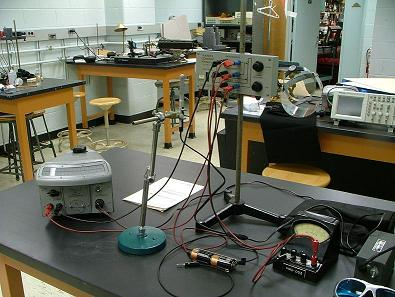
\includegraphics[scale=1.0]{apparatus.png}
\caption{Apparatus \label{fig:setup}}
\end{figure}

\section{Theory}
\indent \indent This section of the manual is clear and concise, with the exception of this passage, "Electrons inside the metal whose energy is less than $K_m_a_x$ will be ejected with less energy." I'm pretty sure they meant to write, "Less than $E_m_a_x$," because electrons inside the metal aren't yet described by some photon energy h$\nu$.

\section{Data}

\begin{figure}[H]
\centering
\hspace{-0.0in}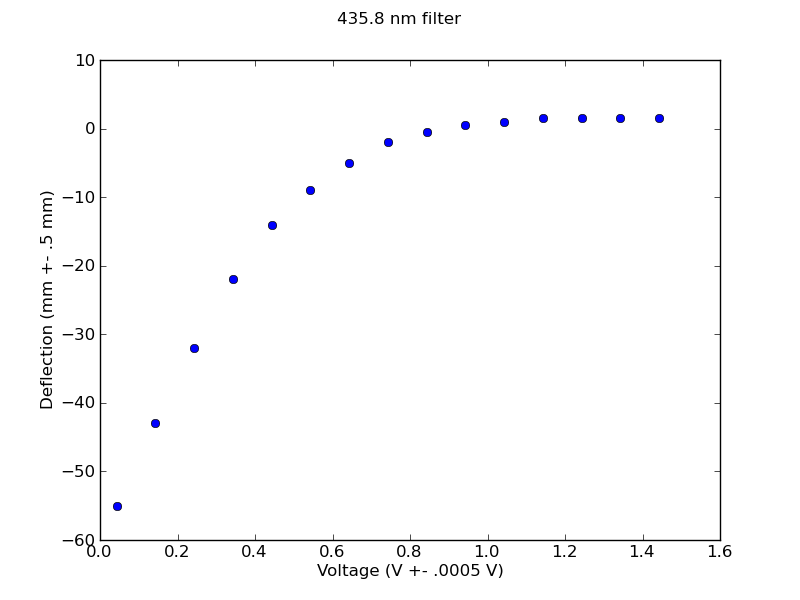
\includegraphics[scale=0.50]{Plot1.png}
\end{figure}

\begin{figure}[H]
\centering
\hspace{-0.0in}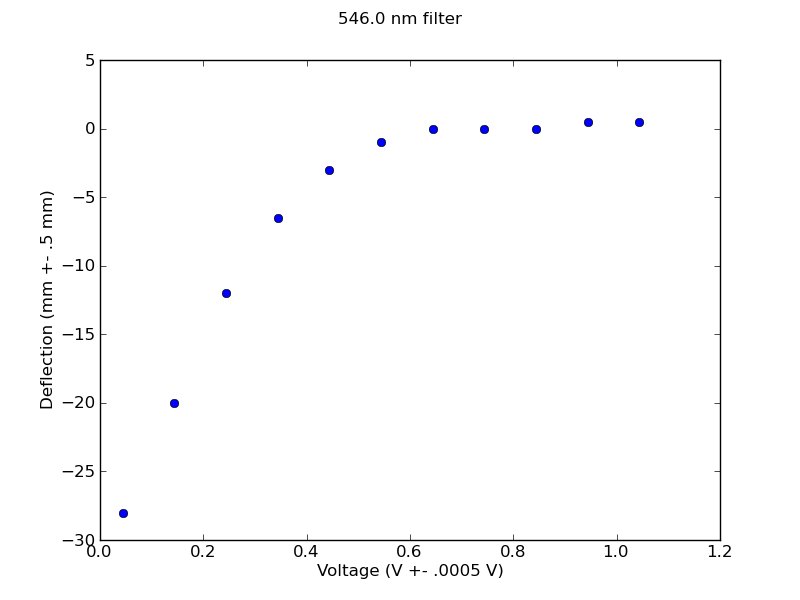
\includegraphics[scale=0.50]{Plot2.png}
\end{figure}

\begin{figure}[H]
\centering
\hspace{-0.0in}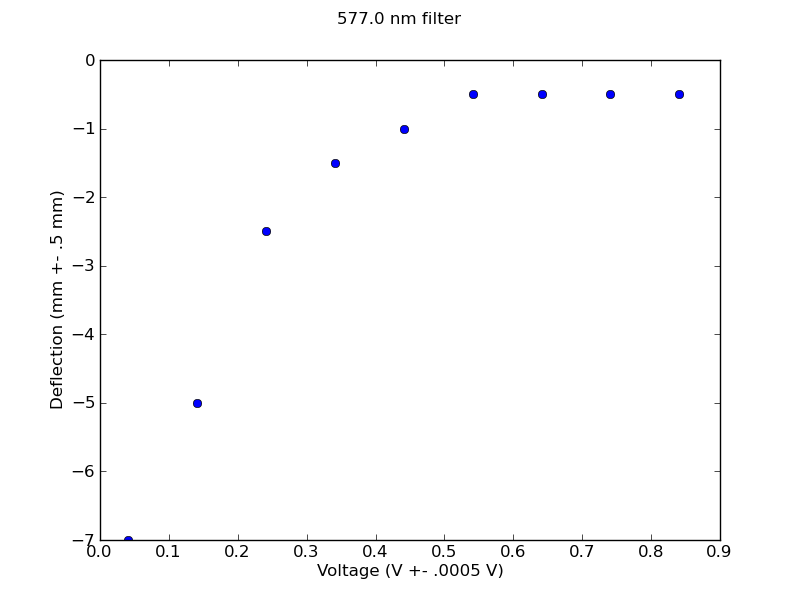
\includegraphics[scale=0.50]{Plot3.png}
\end{figure}

\begin{figure}[H]
\centering
\hspace{-0.0in}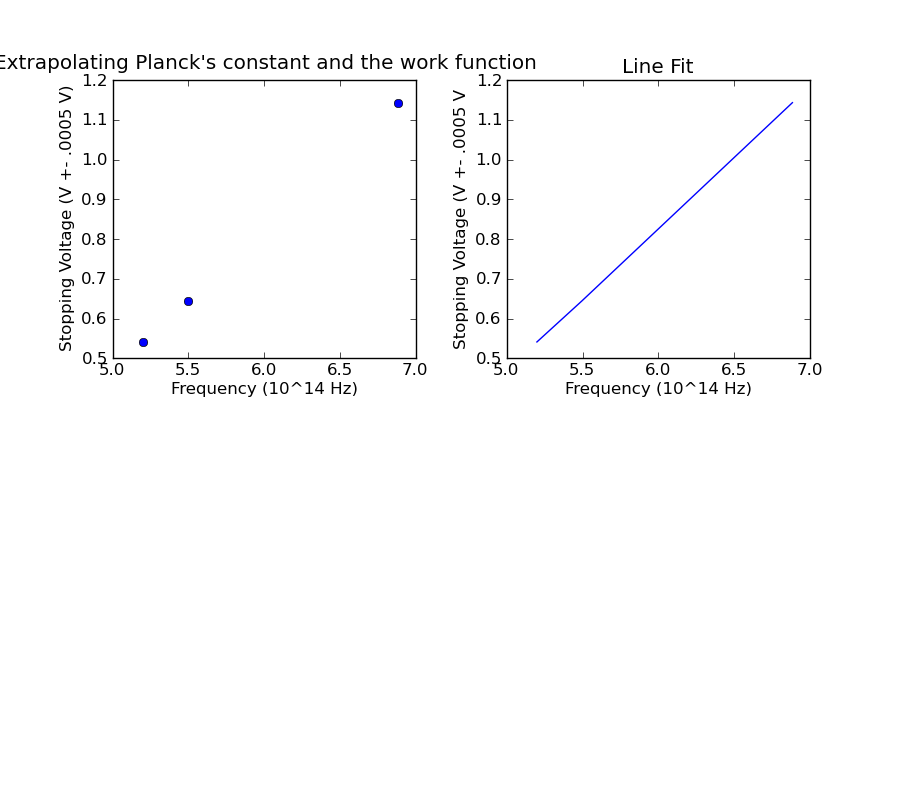
\includegraphics[scale=0.71]{Plot4.png}
\end{figure}

\section{Calculations}
\indent \indent Using the value for the slope of the line fit through stopping voltage plotted against photon frequency:
\[ V_s = \frac{h}{e} \nu - \frac{\phi}{e} \]
\[\frac{h}{e} = 3.579 x 10^-^1^5 \]
\[h = (3.579 x 10^-^1^5)(1.60217646 x 10^-^1^9) = 5.734 x 10^-^3^4 \]

\section{Error Analysis}
\indent \indent There was uncertainty in the voltage and galvanometer The voltage readings were accurate out to three decimal places, so the uncertainty in these readings is $\pm$.0005 V. The distance represented between two ticks on the galvaometer is 1 mm, so the uncertainty in these readings is $\pm$.5 mm.

\[\% Error = \frac{|5.734 x 10^-^3^4 - 6.626 x 10^-^3^4|}{6.626 x 10^-^3^4} = 13.5 \% \]

\section{Conclusion}
\indent \indent I obtained reasonable results and I saw what I expected to see. My result was on the same order of magnitude as the constant I was aiming to calculate, and wasn't very far off. I sufficiently understood this lab.

\section{Questions}
\indent \indent 1. Do the flourescent lights near your lab bench produce an effect? \\
Yes, it produced a deflection of 1 mm to the left of the zero. \\

2. Record the sensitivity of the galvanometer which is pasted on it. \\
110 nominal ohms is the only thing written on the galvanometer. I tried
to find the sensitivity by plugging in the batteries, but the current they
supplied caused a displacement on the galvanometer which was far too large
to read. Sensitivity for galvanometers is defined as some current (usually
in milliamps) per mm.

\end{document}